\section{Experimental Setup}\label{sec:experimental-setup}

Length: 1-2 pages

Explain the overall design of the complete system and list the
configurations (number of middlewares, number of clients, types of
machines, communication patterns) corresponding to the main workloads.

Describe the mechanisms for deploying the system for experiments and the
way performance numbers are gathered and processed. Make the description
so that someone unfamiliar with your system can replicate the steps, and
reference the different script files you submit as code in the SVN
repository.

\subsection{System Configurations}\label{sec:system-configurations}
.	Overall there are three tier components in the system, as it was described in the requirements. The tiers are the database machine, two middleware machines and two client machines. All the machines are t2.medium Amazon EC2 instances. In order to build the Middleware and Client applications Ant was used.
\subsection{Configuration and Deployment mechanisms}\label{sec:configuration-and-deployment-mechanisms}
For configuration of each client as mention in 2.1 the Middleware and the Client were built using Ant. In order to deploy the system including the Database and applications in each tier Python scripts were used. A main script with different function was written in order to perform different operations within the system. Moreover, fabric a python library that works as command line tool and ssh application was used as part of the deployment process.
\subsection{Logging and Benchmarking mechanisms}\label{sec:logging-and-benchmarking-mechanisms}
\begin{figure}[h!]
	\centering
	%\def \svgscale {\columnwidt}
	
\includegraphics[scale=0.3]{logging.png}
	\caption{Different logging entry point during the lifespan of a single request in the messaging system}
	\label{logging}
	%\input{soft-mmu-2.pdf}
\end{figure}
 For the logging mechanism the library lo4j was used. The configuration files is passed as parameter to the Clients and the Middleware application. Both components log the type of request they are preforming, with a timestamp and the number of the request.\\
 
The client just before sending the request make a log entrance and once it get the response enters a second log. In the middleware a log entrance is made when the Middleware gets the request from the client, then when it sends a request to the database and when the request return from it, this one is to estimate the response time of the database from the middleware perspective. Finally after sending the response to the client it enters another log entrance. See Figure \ref{logging}.\\

Finally for benchmarking a python method is the tool is script was written in order to parse the result of the logs provided the middleware and the clients. In addition the middleware has embedded another logging functions to log the throughput of the middleware every second during the execution of it. With those numbers in the log files and the parsing method numbers of the performance of the system were gathered.

\section{Evaluation}\label{sec:evaluation}


\subsection{System Stability}\label{sec:system-stability}

\begin{figure}[h!]
	\centering
	%\def \svgscale {\columnwidt}
	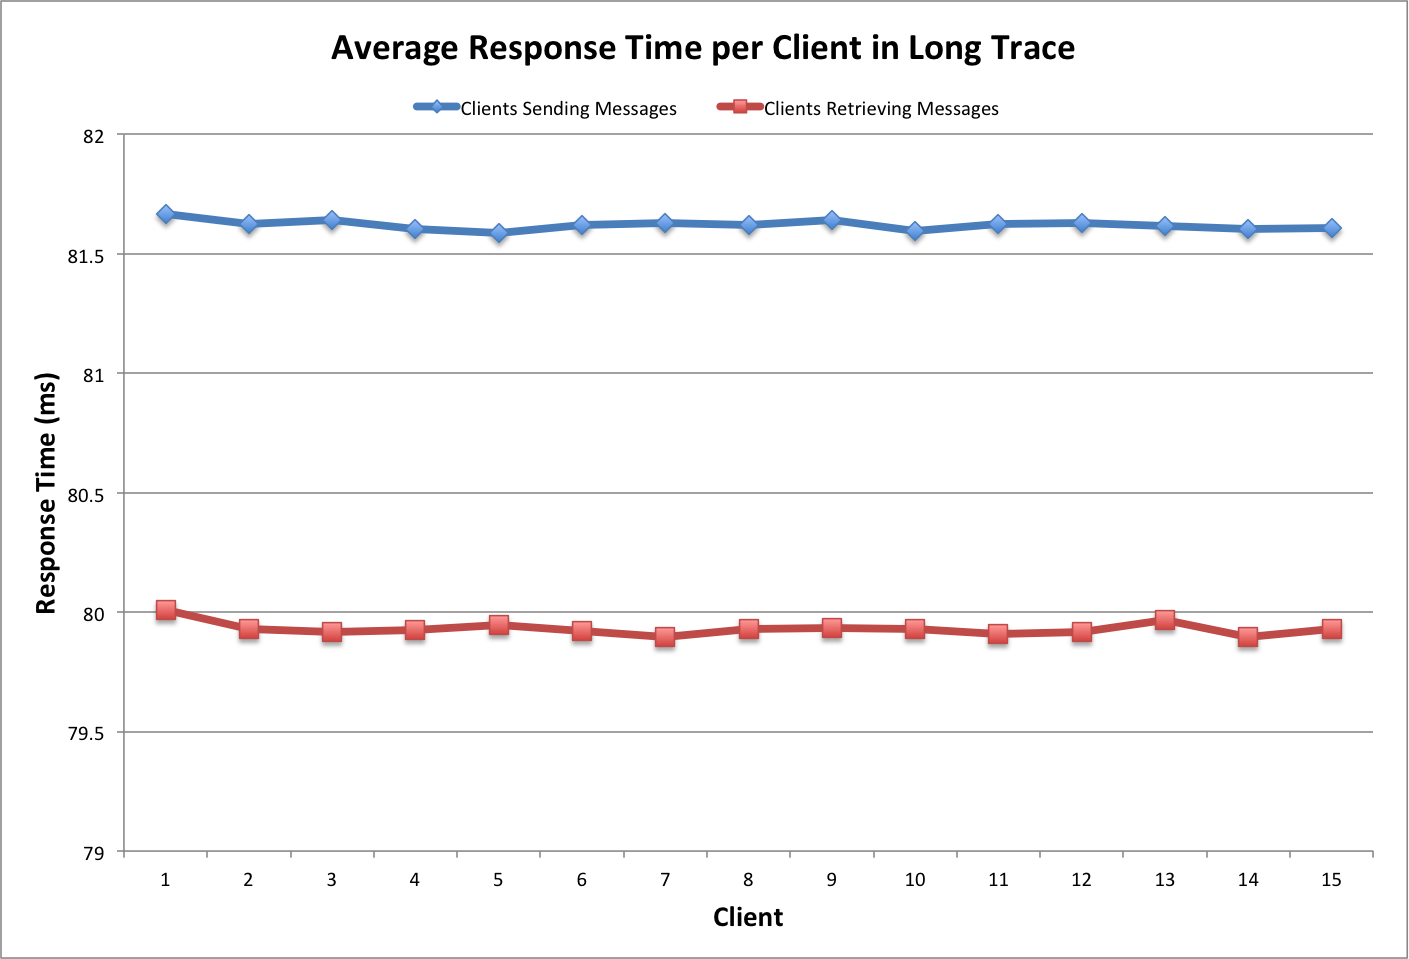
\includegraphics[scale=0.35]{stabilityRP.png}
	\caption{}
	\label{stabilityRP}
	%\input{soft-mmu-2.pdf}
\end{figure}
\begin{figure}[h!]
	\centering
	%\def \svgscale {\columnwidt}
	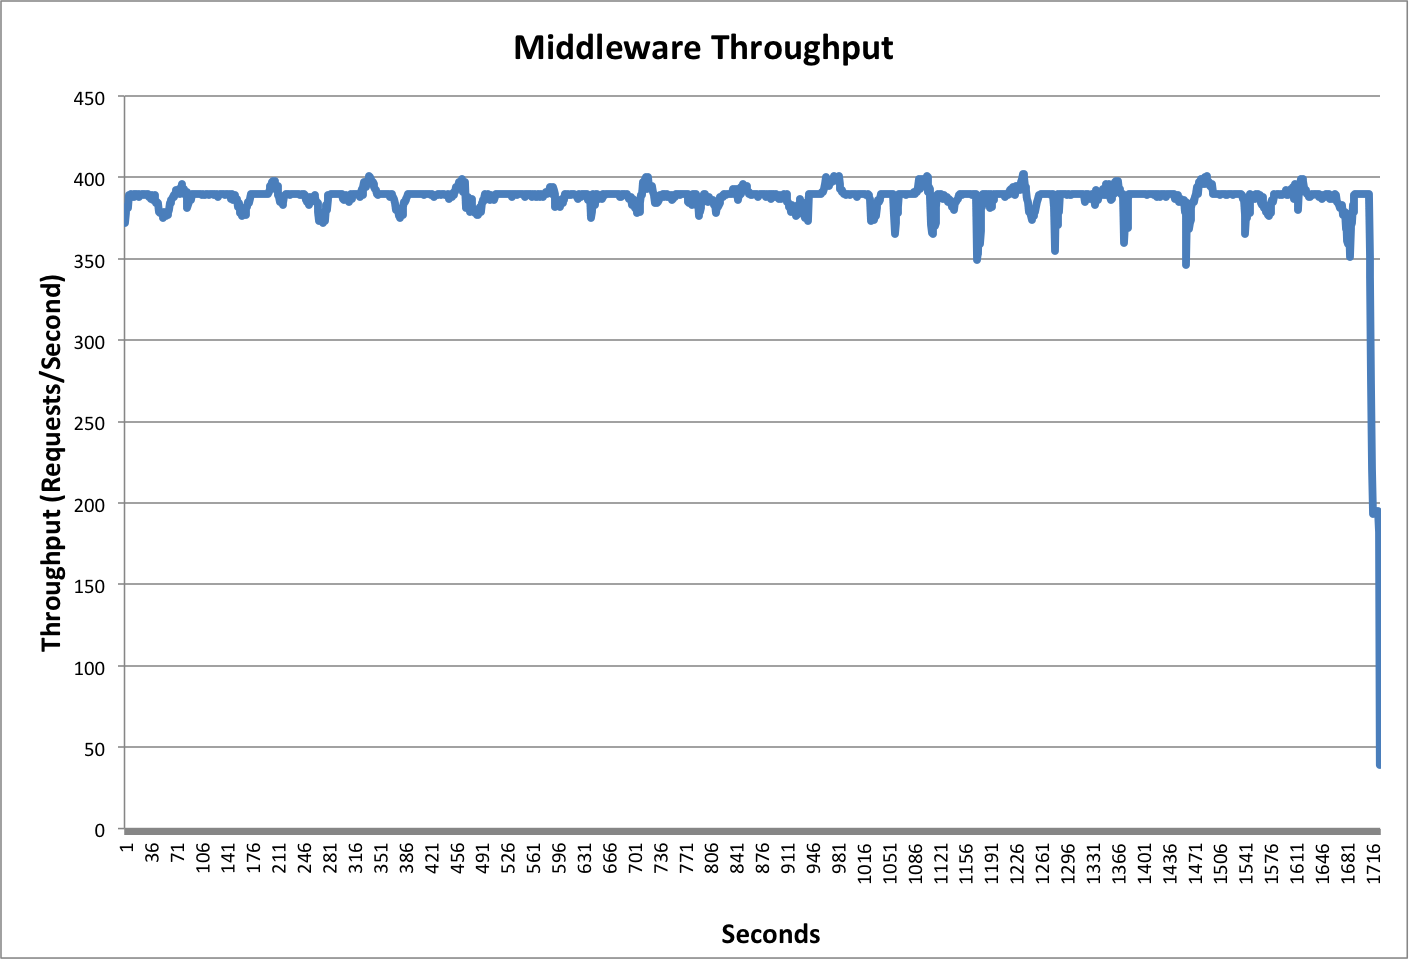
\includegraphics[scale=0.45]{stabilityTHR.png}
	\caption{}
	\label{stabilityTHR}
	%\input{soft-mmu-2.pdf}
\end{figure}
\subsection{System Throughput}\label{sec:system-throughput}

\begin{figure}[h!]
	\centering
	%\def \svgscale {\columnwidt}
	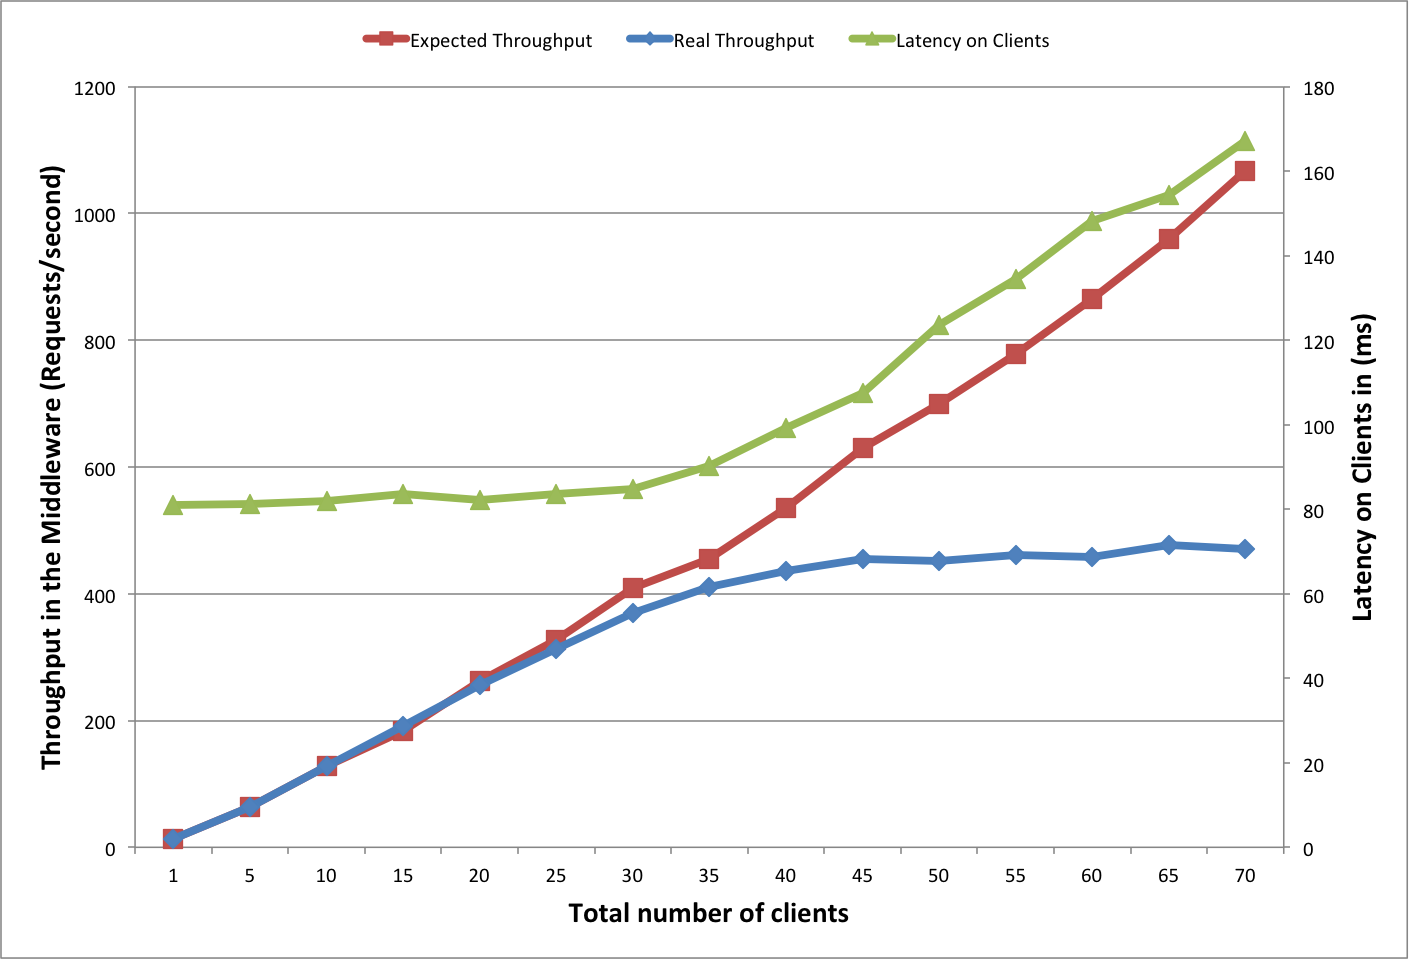
\includegraphics[scale=0.4]{through.png}
	\caption{}
	\label{through}
	%\input{soft-mmu-2.pdf}
\end{figure}

\subsection{System Scalability}\label{sec:system-scalability}



\subsection{Response Time Variations}\label{sec:response-time-variations}



\subsection{$2^k$ Experiment}\label{sec:k-experiment}
For the 2\^{}k experiment the two factors I decided to explore ere the number of concurrent client in my middleware (Handlers) and my number of connections in the database, the reason was because as I observed in my through put experiment by increasing the number of clients allowed in the system in the handler parameter the throughput was increasing. Furthermore I wanted to see the impact on the number of connection in the system.\\

Both parameters were explored in two levels each with the values of 10 and 20. As result I had to preform the experiment 4 times with adjusting the values of the previous parameters. Each experiment was running for 10 minutes, with t2.medium instances each client with and average workload of 12 requests per second.
By performing this experiment we are able to see the impact of these factors in the performance of the system in Request completed by second (Req/sec).

After the data seen in Table \ref{2k}, I define my two variables $x_{a}$ and $x_{b}$



\begin{table*}\centering
         % \ra{1.3}
         % \tabcolsep=0.5cm
         \scalebox{0.8}{
         \begin{tabular}{@{}rrcc@{}}
                  \toprule
                    & \multicolumn{3}{c}{Connection to Database} \\
                  \cmidrule{2-4}
                   \multicolumn{1}{c}{$Client Hanlder$} &&$10$ &$20$\\
                  \midrule 
			         10 &&$129.354782609$&$128.763478261$   \\
			          20 &&$257.597560976$&$258.93554007$   \\
                  \bottomrule
                  \end{tabular}
         }
         \caption{}
         \label{2k}
 \end{table*}  
 
 $$x_{a}=\begin{cases} -1& if\quad 10 \quad Connections\quad  to\quad  Dabatase\\1 & if\quad 20 \quad Connections\quad  to\quad  Dabatase\end{cases}\\
 $$
 $$x_{b}=\begin{cases} -1& if\quad 10 \quad Client\quad Hanlders\\1 & if\quad 20 \quad Client\quad Hanlders\end{cases}$$
 After the analysis of my result my hypothesis about the number of Client Handler impacting in high way the performance of my system is true. Furthermore I was able to show that given the current configuration of my database and the number of connections it has is more than enough for my system.\\
 
Furthermore my $2^k$ experiment show that the mean request per second is $193.6628405$, also the impact of the connection in request per second of my database connections is very low $ 0.186668686$ requests per second. However the value in my number of Client Handlers account for $ 64.60371004$ Requests per second. Finally the interaction of these two combined have an effect of $ 0.482320861$ Request per Second.See Table \ref{2kr}.


\begin{table*}\centering
         % \ra{1.3}
         % \tabcolsep=0.5cm
         \scalebox{0.8}{
         \begin{tabular}{@{}rrrrr@{}}
         \toprule
         
          & \multicolumn{3}{c}{Design of $2^2$ Experiment} \\
         \cmidrule{1-5}

         I           & A           & B           & AB          & y           \\
         \midrule 
         1           & -1          & -1          & 1           & 129.3547826 \\
         1           & 1           & -1          & -1          & 128.7634783 \\
         1           & -1          & 1           & -1          & 257.597561  \\
         1           & 1           & 1           & 1           & 258.9355401 \\
         774.6513619 & 0.746674746 & 258.4148402 & 1.929283442 & Total       \\
         193.6628405 & 0.186668686 & 64.60371004 & 0.482320861 & Total/4  \\
         \bottomrule  
         \end{tabular}
         }
         \caption{}
         \label{2kr}
         
 \end{table*}  

\subsection{Conclusion}\label{sec:conclusion}
